\documentclass[10pt,landscape,a4paper]{article}
\usepackage[utf8]{inputenc}
\usepackage[ngerman]{babel}
\usepackage[T1]{fontenc}
%\usepackage[LY1,T1]{fontenc}
%\usepackage{frutigernext}
%\usepackage[lf,minionint]{MinionPro}
\usepackage{tikz}
\usetikzlibrary{shapes,positioning,arrows,fit,calc,graphs,graphs.standard}
\usepackage[nosf]{kpfonts}
\usepackage[t1]{sourcesanspro}
\usepackage{multicol}
\usepackage{wrapfig}
\usepackage[top=0mm,bottom=1mm,left=0mm,right=1mm]{geometry}
\usepackage[framemethod=tikz]{mdframed}
\usepackage{microtype}
\usepackage{pdfpages}
\usepackage{amsmath}

\let\bar\overline

\definecolor{myblue}{cmyk}{1,.72,0,.38}

\def\firstcircle{(0,0) circle (1.5cm)}
\def\secondcircle{(0:2cm) circle (1.5cm)}

\colorlet{circle edge}{myblue}
\colorlet{circle area}{myblue!5}

\tikzset{filled/.style={fill=circle area, draw=circle edge, thick},
    outline/.style={draw=circle edge, thick}}
    
\pgfdeclarelayer{background}
\pgfsetlayers{background,main}

\everymath\expandafter{\the\everymath \color{myblue}}
\everydisplay\expandafter{\the\everydisplay \color{myblue}}

\renewcommand{\baselinestretch}{.8}
\pagestyle{empty}

\global\mdfdefinestyle{header}{%
linecolor=gray,linewidth=1pt,%
leftmargin=0mm,rightmargin=0mm,skipbelow=0mm,skipabove=0mm,
}

\newcommand{\header}{
\begin{mdframed}[style=header]
\footnotesize
\sffamily
Econometrics Year 1 Cheat-sheet\\
~Julian~Budde,~Page~\thepage~of~2
\end{mdframed}
}

\makeatletter % Author: https://tex.stackexchange.com/questions/218587/how-to-set-one-header-for-each-page-using-multicols
\renewcommand{\section}{\@startsection{section}{1}{0mm}%
                                {.2ex}%
                                {.2ex}%x
                                {\color{myblue}\sffamily\small\bfseries}}
\renewcommand{\subsection}{\@startsection{subsection}{1}{0mm}%
                                {.2ex}%
                                {.2ex}%x
                                {\sffamily\bfseries}}



\def\multi@column@out{%
   \ifnum\outputpenalty <-\@M
   \speci@ls \else
   \ifvoid\colbreak@box\else
     \mult@info\@ne{Re-adding forced
               break(s) for splitting}%
     \setbox\@cclv\vbox{%
        \unvbox\colbreak@box
        \penalty-\@Mv\unvbox\@cclv}%
   \fi
   \splittopskip\topskip
   \splitmaxdepth\maxdepth
   \dimen@\@colroom
   \divide\skip\footins\col@number
   \ifvoid\footins \else
      \leave@mult@footins
   \fi
   \let\ifshr@kingsaved\ifshr@king
   \ifvbox \@kludgeins
     \advance \dimen@ -\ht\@kludgeins
     \ifdim \wd\@kludgeins>\z@
        \shr@nkingtrue
     \fi
   \fi
   \process@cols\mult@gfirstbox{%
%%%%% START CHANGE
\ifnum\count@=\numexpr\mult@rightbox+2\relax
          \setbox\count@\vsplit\@cclv to \dimexpr \dimen@-1cm\relax
\setbox\count@\vbox to \dimen@{\vbox to 1cm{\header}\unvbox\count@\vss}%
\else
      \setbox\count@\vsplit\@cclv to \dimen@
\fi
%%%%% END CHANGE
            \set@keptmarks
            \setbox\count@
                 \vbox to\dimen@
                  {\unvbox\count@
                   \remove@discardable@items
                   \ifshr@nking\vfill\fi}%
           }%
   \setbox\mult@rightbox
       \vsplit\@cclv to\dimen@
   \set@keptmarks
   \setbox\mult@rightbox\vbox to\dimen@
          {\unvbox\mult@rightbox
           \remove@discardable@items
           \ifshr@nking\vfill\fi}%
   \let\ifshr@king\ifshr@kingsaved
   \ifvoid\@cclv \else
       \unvbox\@cclv
       \ifnum\outputpenalty=\@M
       \else
          \penalty\outputpenalty
       \fi
       \ifvoid\footins\else
         \PackageWarning{multicol}%
          {I moved some lines to
           the next page.\MessageBreak
           Footnotes on page
           \thepage\space might be wrong}%
       \fi
       \ifnum \c@tracingmulticols>\thr@@
                    \hrule\allowbreak \fi
   \fi
   \ifx\@empty\kept@firstmark
      \let\firstmark\kept@topmark
      \let\botmark\kept@topmark
   \else
      \let\firstmark\kept@firstmark
      \let\botmark\kept@botmark
   \fi
   \let\topmark\kept@topmark
   \mult@info\tw@
        {Use kept top mark:\MessageBreak
          \meaning\kept@topmark
         \MessageBreak
         Use kept first mark:\MessageBreak
          \meaning\kept@firstmark
        \MessageBreak
         Use kept bot mark:\MessageBreak
          \meaning\kept@botmark
        \MessageBreak
         Produce first mark:\MessageBreak
          \meaning\firstmark
        \MessageBreak
        Produce bot mark:\MessageBreak
          \meaning\botmark
         \@gobbletwo}%
   \setbox\@cclv\vbox{\unvbox\partial@page
                      \page@sofar}%
   \@makecol\@outputpage
     \global\let\kept@topmark\botmark
     \global\let\kept@firstmark\@empty
     \global\let\kept@botmark\@empty
     \mult@info\tw@
        {(Re)Init top mark:\MessageBreak
         \meaning\kept@topmark
         \@gobbletwo}%
   \global\@colroom\@colht
   \global \@mparbottom \z@
   \process@deferreds
   \@whilesw\if@fcolmade\fi{\@outputpage
      \global\@colroom\@colht
      \process@deferreds}%
   \mult@info\@ne
     {Colroom:\MessageBreak
      \the\@colht\space
              after float space removed
              = \the\@colroom \@gobble}%
    \set@mult@vsize \global
  \fi}

\makeatother
\setlength{\parindent}{0pt}

\begin{document}
%\footnotesize
\footnotesize
\begin{multicols*}{5}
\section{Probability Theory}
\textbf{Theorem 1.3}: $A_1, ..., A_2$ partition of $S$ and $B\subset S$, then $P(B) = \sum_{i=1}^\infty P(B|A_i)P(A_i)$.
\section{Random Variables}
\textbf{Thm 2.5 (Jensen's inequalities)}: Suppose $g(x)$ convex, then $E(g(X)) \geq g(E(X))$ if existent. Strict unless $X$ degenerate or $g$ linear.\\
\textbf{Def 2.10 (MGF)}: $X\sim F_X$, $t\in\mathbb{R}$. Then $M_X(t) = E(e^{tX})$ given it exists in some neighborhood of 0.\\
\textbf{Thm 2.7}: If $M_X(t)$ exists, then $E(X^n) = \frac{\partial^n}{\partial t^n}M_X(0)$. % Derive by writing out (continuous).\\

\section{Multivariate Distributions}
\textbf{Def 3.1}: $n$-dimensional rvec is $f: S \to \mathbb{R}^n$.\\
\subsection{Bivariate Random Vectors}
Define probability functions on Borel sigma algebra of $\mathbb{R}^2$.\\
% \textbf{Joint CDF}: $F_{X,Y}(x,y) = P(X\leq x, Y\leq y)$.\\
% \textbf{Joint PMF (discrete (X,Y))}: $f_{X,Y} = P(X=x, Y=y)$.\\
% \textbf{Joint PDF (cont + diff)}: $f_{X,Y} = \frac{\partial^2}{\partial x\partial y}F_{X,Y}(x,y)$.\\
% \textbf{Joint PDF (cont + not diff everywhere)}: implicitly via $F_{X,Y} = \int_{-\infty}^y\int_{-\infty}^xf_{X,Y}(u,v)dudv$. \\
% \textbf{Expectations (discrete)}: $E(g(X,Y)) = \sum_{(x,y)\in\mathbb{R}^2:f_{X,Y}(x,y)>0}g(x,y)f_{X,Y}(x,y)$.\\
% \textbf{Expectations (continuous)}: $E(g(X,Y)) = \int_{-\infty}^\infty\int_{-\infty}^\infty g(x,y)f_{X,Y}(x,y)dxdy$.\\
Need to assume $E(|g(X,Y)|) < \infty$.\\
% \textbf{Discrete-Continuous Case}: Define wrt Borel sigma algebra.\\
\textbf{Joint $\Rightarrow$ Marginal}: $F_X(x) = lim_{y\to\infty}F_{X,Y}(x,y)$ and $f_{X}(x) = \int_{-\infty}^\infty f_{X,Y}(x,v)dv$.\\

\subsection{Continuous Distributions}
%\textbf{Conditional PMF}: $f_{Y|X}(y|x) = P(Y=y|X=x) = \frac{f_{X,Y}(x,y)}{f_X(x)}$.\\
%\textbf{Conditional CDF (discrete)}: $F_{Y|X}(y|x) = P(Y\leq y|X=x) = \frac{P(Y\leq Y, X = X)}{P(X=x)}$.\\
%For continuous rvs more difficult because $P(X=x) = 0$.\\
%\textbf{Conditional CDF (continuous)}: $F_{Y|X}(y|x) = \lim_{\epsilon\downarrow0}P(Y\leq y | X \in [x-\epsilon, x + \epsilon]) = \ldots = \int_{-\infty}^y \left(\frac{f_{X,Y}(x,v)}{f_X(x)}\right)dv$, which also implies cond pdf.\\
\textbf{Conditional Expectation}: $E(g(Y)|X=x) = \sum_{y\in\mathbb(Y)}g(y)f_{Y|X}(y|x)$ or $=\int_{-\infty}^\infty g(y)f_{Y|X}(y|x)dy$.\\
\textbf{Thm 3.1 (LIE)}: $Y,X$ rvs, then $E(Y) = E_X(E_{Y|X}(Y|X))$.\\
\textbf{Law of iterated variance}: $Var(Y) = E(Var(Y|X)) + Var(E(Y|X))$.

\subsection{Independence}
\textbf{Def 3.4}: $(X,Y)$ rvec, $X,Y$ \textit{independent} if $\forall x\in \mathbb{R}, y\in\mathbb{R}$ we have $f_{X,Y}(x,y) = f_X(x)f_Y(y)$.\\
\textbf{Thm 3.2}: $X,Y$ independent $\Leftrightarrow$ for any two bounded $g,h:\mathbb{R}\to\mathbb{R}$ we have $E(g(X)g(Y)) = E(g(X))E(h(Y))$.\\
\textbf{Thm 3.3}: $X,Y$ independent, $g(X)$ and $g(Y)$ independent.\\

%\subsection{Measure of linear relationships}
%\textbf{Covariance}: $Cov(X,Y) = E[(X-E(X))(Y-E(Y))]$.\\
%\textbf{Independence and Cov}: Independence $\Rightarrow Cov(X,Y) = 0$, but not the other way around (e.g. $X~\sim Unif(-1,1), Y=X^2$).\\
%\textbf{Correlation}: $Corr(X,Y) = \frac{Cov(X,Y)}{SD(X)SD(Y)} \in [-1,1]$.\\
 



\section{Sampling}
\section{Asymptotic Theory}
\subsection{Inequalities}
\textbf{Thm 5.1 (Markov's Inequality)}: $X$ r.v., $g: \mathbb{R} \to [0, \infty)$, then $\forall \epsilon > 0$, $P(g(X) > \epsilon) \leq \frac{E(g(X))}{\epsilon}$.\\
\textbf{Cor 5.1 (Chebyshev's Inequality)}: $X$ r.v., then $\forall \epsilon > 0$, $P(|X-E(X)| \geq \epsilon) \leq \frac{Var(X)}{\epsilon^2}$.

\subsection{Modes of Convergence}
\textbf{Def 5.2}: $plim_{n\to\infty}X_n = X \leftrightarrow \lim_{n\to\infty}P(|X_n-X|<\epsilon) = 1$.\\
%\textbf{Def 5.3}: $\hat{\theta}_n \emph{consistent} for \theta \leftrightarrow plim\hat{\theta}_n = \theta$. \\
\textbf{Def 5.4}: $\{X_n\}_{n=1}^\infty$ converges in \emph{distribution} to $X$ $\leftrightarrow$ $\lim_{n\to\infty}F_{X_n}(x) = F_X(x)$ for every continuity point of $x$ of $F_X(\cdot)$. \\
\textbf{Def 5.5}: $\{X_n\}_{n=1}^\infty$ converges in \emph{mean square} to $X$ $\leftrightarrow$ $\lim_{n\to\infty}E[(X_n-X)^2] = 0$. \\
\textbf{Thm 5.2}: $X_n \xrightarrow{m.s.} \Rightarrow X_n \xrightarrow{p}X$. Proof by Chebyshev's inequality. The reverse is not true, consider $X_n \in{0, \sqrt{n}}$ with probabilities $1-1/n, 1/n$.\\
\textbf{Thm 5.3}: $X_n \xrightarrow{p} \Rightarrow X_n \xrightarrow{d}X$. Proof uses definition of $\xrightarrow{p}$ and continuity. The reverse is generally \emph{not true}, consider $X_n = Z \sim N(0,1)$ and $X, Z \sim N(0, 1)$, have $F_{X_n}(x) = F_X(x)$ but $P(|Z-X|\geq\epsilon) > 0$. Exception: $X_n \xrightarrow{d} c \in \mathbb{R} \Rightarrow X_n \xrightarrow{p} c$.

\subsection{Law of Large Numbers}
%\textbf{Thm 5.4 (LLN)}: ${X_i}_{i=1}^\infty$ seq. of uncorrelated rvs from $F_X$ with $\mu = E(X)$, $Var(X)$ existing and finite. Then $\bar{X}_n \xrightarrow{p}\mu$. Proof: Chebyshev's inequality.\\
%\textbf{Thm 5.5 (WLLN)}: ${X_i}_{i=1^\infty}$ seq. of uncorrelated rvs. Suppose $\mu_i = E(X_i)$ and $\sigma_i^2 = Var(X_i)$ exist and finite. If $\lim_{n\to\infty}\frac{1}{n^2}\sum_{i=1}^n\sigma_i^2 = 0$ then $\bar{X}_n - \frac{1}{n}\sum_{i=1}^n\mu_i \xrightarrow{p} 0$. \\
\textbf{Thm 5.6 (LLN i.i.d)}: $\{X_i\}_{i=1}^\infty$ seq. of iid rvs from $F_X$ with $\mu=E(X)$ exist and finite. Then $\bar{X}_n\xrightarrow{p}\mu$.\\
\textbf{Convergence Criteria}: Need a combination of three assumptions: (1) finite mean and/or variance (no LLN for Cauchy), (2) bounds on asymptotic variance (e.g. not growing too fast with $i$), (3) restricted dependence.

\subsection{Central Limit Theorem}
\textbf{Thm 5.7 (Lindeberg-Levy CLT)}: $\{X_i\}_{i=1}^\infty$ seq. of iid rvs from $F_X$, $\mu$ and $\sigma^2$ finite. Then $\sqrt{n}(\bar{X}_n-\mu) \xrightarrow{d} N(0,\sigma^2)$. \\
\textbf{Thm 5.9 (Berry-Esseen)}: $\{X_i\}_{i=1}^\infty$ seq. of iid rvs from $F_X$, $\mu$ and $\sigma^2$ finite and $\lambda = E(|X-E(X)|^3)$ exist and finite. Let $Z\sim N(0,1)$. Then $|P\left(\frac{\sqrt{n}(\bar{X}_n-\mu)}{\sigma}\leq x\right) - P(Z\leq x)| \leq \frac{C\lambda}{\sigma^3\sqrt{n}}$.\\

\subsection{Convergence of Random Vectors}
\textbf{Def 5.7}: $\textbf{X}_n \xrightarrow{p} \textbf{X} \leftrightarrow \lim_{n\infty}P(||\textbf{X}_n - \textbf{X}||<\epsilon)=1$.\\
\textbf{Def 5.8}: $\textbf{X}_n \xrightarrow{ms} \textbf{X} \leftrightarrow \lim_{n\infty}E(||\textbf{X}_n - \textbf{X}||^2)=0$.\\
\textbf{Def 5.9}: $\textbf{X}_n \xrightarrow{d} \textbf{X} \leftrightarrow \lim_{n\infty}F_{\textbf{X}_n}(x) = F_\textbf{X}(x)$ for every continuity point $x$ of $F_\textbf{X}(\cdot)$.\\
\textbf{Thm 5.10 (Cramér-Wold)}: $\{\textbf{X}_n\}_{n=1}^\infty$ seq. of K-dimensional random vectors. Then, $\forall \lambda\in\mathbb{R^K}$ we have $\lambda'\textbf{X}_n \xrightarrow{d} \lambda'\textbf{X}$ $\leftrightarrow$ $\textbf{X}_n \xrightarrow{d} \textbf{X}$.

\subsection{CMT and Slutzky's}
\textbf{Thm 5.11 (CMT)}: Let $\{\textbf{X}_n\}_{n=1}^\infty$ be a sequence of K-dim. rvecs $\textbf{X}$ K-dim rvec, and $g:\mathbb{R^K}\to\mathbb{R}$ with discontinuity points D such that $P(\textbf{X}\in D)=0$. \\
(a) $\textbf{X}_n \xrightarrow{p} \textbf{X} \Rightarrow g(\textbf{X}_n) \xrightarrow{p} g(\textbf{X})$.\\
(b) $\textbf{X}_n \xrightarrow{d} \textbf{X} \Rightarrow g(\textbf{X}_n) \xrightarrow{d} g(\textbf{X})$. \\
Implication: Sums and products of convergent sequences converge. Does \emph{not} hold for \emph{mean square} convergence.\\
\textbf{Thm 5.12 (Slutzky's)}: $X_n$, $Y_n$ seq of rvs with $X_n\xrightarrow{d} X$ and $Y_n\xrightarrow{p} c\in \mathbb{R}$, then $X_n + Y_n \xrightarrow{d} X + c$ and $X_nY_n\xrightarrow{d}cX$, and if $c\neq0$, $X_n/Y_n \xrightarrow{d} X/c$. \\
\textbf{Extension to rvecs}: $\textbf{X}_n \xrightarrow{d} \textbf{X}$ and $\textbf{Y}_n\xrightarrow{p}\textbf{C}\in\mathbb{R}^{K\times K}$, $\textbf{C}$ invertible, then $\textbf{Y}_n^{-1}\textbf{X}_n\xrightarrow{d}\textbf{C}^{-1}\textbf{X}$. \\
\textbf{Example CMT}: $\left(\frac{\sqrt{n}(\bar{X}_n - \mu)}{\sigma}\right)^2 \xrightarrow{d} N(0,1)^2 = \chi_1^2$.\\
\textbf{Thm 5.13 (Delta-Method)}: $X_n$ seq of rvs with LL-CLT applying. $g:\mathbb{R}\to\mathbb{R}$ \emph{continuously diff.} at $\mu$ with $g'(\mu)\neq0$. Then $\sqrt{n}(g(X_n)-g(\mu)) \xrightarrow{d} N(0, g'(\mu)^2\sigma^2)$. Proof: CMT and Slutzky's applied to Taylor's/intermediate value theorem. 

\subsection{Interval Estimation}
Suppose $\{X_i\}_{i=1}^n$ is a seq of iid random variables with $\mu, \sigma^2$ finite. Then an asymptotically valid CI for $\mu$ is given by 
$CI = \left[\bar{X}_n \pm \frac{z_{1-\alpha/2}}{\sqrt{n}}S_n\right]$
where $S_n$ is a consistent estimator of $\sigma$ and $P(\mu\in CI) \to 1-\alpha$. Proof: CLT, CMT, Slutzky. 

\subsection{Moment-Based Estimation}
\textbf{Parameter of interest}: $\theta = h(E(g(X)))$ (simple case: $X, \theta$ scalars and $g:\mathbb{R}\to\mathbb{R}$ and $h:\mathbb{R}\to\mathbb{R}$ cont. diff.).\\
\textbf{Moment-based estimator}: $\hat{\theta}_n = h\left(\frac{1}{n}\sum_{i=1}^ng(X_i)\right)$. \emph{Consistency}: LLN and CMT. \\
\textbf{Large-sample distribution}: If $Var(g(X))<\infty$ CLT applies so $\sqrt{n}\left(\frac{1}{n}\sum_{i=1}^ng(X_i) - E(g(X))\right)\xrightarrow{d}N(0, Var(g(X)))$. By the \emph{delta-method} if $h'(g(E(X)))\neq0$ we have 
$		\sqrt{n}(\hat{\theta}_n - \theta) = 
		%\sqrt{n}\left(h\left(\frac{1}{n}\sum_{i=1}^ng(X_i)\right) - h(E(g(X)))\right) \\
		\xrightarrow{d} N(0, h'(E(g(X))^2Var(g(X)))).$

\section{Maximum Likelihood Estimation}
\textbf{Def 6.1 (likelihood function)}: $L_n(\theta) = \prod_{i=1}^nf(\textbf{x}_i;\theta)$.\\
Equivalently, we define the \textit{log-likelihood function} as $\log(L_n(\theta))$.\\
\textbf{Thm 6.1}: Suppose $\textbf{X}$ is a random vector with pdf or pmf $f(\textbf{x};\theta_0)$. Then $E(\log(f(\textbf{x};\theta)))\geq E(ln(f(\textbf{X};\theta))), \forall \theta in \Theta$.\\
\textbf{Thm 6.2}: For $\tau(\theta)$ and $\hat{\theta}_n$ MLE of $\theta$, we have $\tau(\hat{\theta}_n)$ is MLE of $\tau(\theta)$.

\subsection{Distribution of the MLE}
\textbf{MLE Limit Distribution}: $\sqrt{n}(\hat{\theta}_n - \theta) \xrightarrow{d} N(0, A^{-^1}BA^{-1})$ with $A = E_\theta[-\frac{\partial^2}{\partial\theta\partial'\theta}ln(f(\textbf{X}_i);\theta)]$ and $B = E_\theta[\frac{\partial}{\partial\theta}ln(f(\textbf{X}_i;\theta))\frac{\partial}{\partial\theta'}ln(f(\textbf{X}_i;\theta))]$. B \textit{var-cov} matrix of the score (since score mean zero by FOC). A is \textit{Fisher information}.\\
\textbf{Thm 6.3}: Under weak reg. cond. (diff; interch. integr./diff.) we have $A=B$.

\subsection{CRLB}
We could try to define "best" estimator in terms of MSE. However, MSE might depend on $\theta$ (e.g. $\bar{X}_n$ vs. $1$, the latter dominates for $\theta = 1$).\\
Progress: Focus on \textit{unbiased} estimators and thus variance.\\
\textbf{Thm 6.4}: $\{X_i\}$ rs from $f(\textbf{x};\theta)$, $\hat{\theta}_n$ estimator of $\theta$. Then under some reg conds $Var_\theta[\hat{\theta}_n] = \frac{(\frac{\partial}{\partial\theta}E_\theta[\hat{\theta}_n])^2}{nE_\theta[(\frac{\partial}{\partial\theta}\log(f(\textbf{X};\theta)))^2]}$.\\
With unbiased estimators (numerator equals one) estimators attaining the lower bound are called \textit{efficient}.\\
Caveats: (1) Finite-sample efficient estimators rare; even MLE often biased, (2) allowing some bias can reduce variance and thus MSE, (3) MSE might not be criterion of interest.\\
\textbf{Relative efficiency}: $E_\theta[(\hat{\theta}_{1,n}-\theta)^2] \leq E_\theta[(\hat{\theta}_{2,n}-\theta)^2]$ for all $\theta\in\Theta$ and strict for some.\\
\textbf{Asymptotic efficiency}: Asymptotic distribution often implies \textit{asymptotically unbiased}, efficiency than means attaining CRLB asymptotically. Thus, the MLE is asymptotically efficient. Similar, for two estimators (possibly not attaining the CRLB) we can say one is \textit{asymptotically relatively more efficient} (i.e. has lower asymptotic variance).
\section{Hypothesis Testing}
\subsection{Basics}
\textbf{Def 7.1}: A \emph{hypothesis} is a statement about the population distribution.\\
\textbf{Def 7.2}: $H_0$ (null hypothesis) and $H_1$ (alternative hypothesis) are the complementary hypothesis. We write $H_0:\theta\in\Theta_0$ and $H_1:\theta\in\Theta_1$ with $\Theta_k$ mutually exclusive and exhaustive.\\
\emph{Simple} hypothesis: $\Theta_0$ is singleton. \emph{Composite} hypothesis: $\Theta_1$ more than one value.\\
\textbf{Def 7.3}: A \emph{hypothesis test} is a rule when to reject $H_0$ (in favor of $H_1$) given the data. \footnotesize{(\textit{Accepting} $H_0$ is weird, e.g. what about $\theta_0+\epsilon$?.)}\\

\section{Size and Power}
\textbf{Type-I error}: Reject $H_0$ although in fact true.\\
\textbf{Type-II error}: \emph{Not} reject $H_0$ although in fact false.\\
\textbf{Error rates}: \emph{Probabilities} of making these errors \footnotesize{(errors are random because they depend on the sample)}.\\
\textbf{I-II-trade-off}: We want to minimize $P_\theta(reject H_0)$ $\forall \theta\in\Theta_0$ and maximize $P_\theta(reject H_0)$ $\forall \theta\in\Theta_1$ \footnotesize{($P_\theta$ denotes probabilities assuming $\theta$ is the true parameter).}\\
\textbf{Def 7.4 (Power function)}: $\beta(\theta) = P_\theta(reject H_0)$.\\
\textbf{Type-I error}: $\beta(\theta)$ for any $\theta\in\Theta_0$.\\
\textbf{Type-II error}: $\beta(\theta)$ for any $\theta\in\Theta_1$.\\
\textbf{Def 7.5/7.6}: For $\alpha\in[0,1]$, a test is \emph{level} $\alpha$ if $\sum_{\theta\in\Theta_0}\beta(\theta)\leq\alpha$ (\emph{size}: equality).\\
\textbf{Test choice}: One approach: fix $\alpha$, take the one with the best power over all $\theta\in\Theta_1$ (might not exist).\\

\subsection{Test statistics and critical values}
\textbf{Goal}: Derive statistic $T$ and reject iff $T>c_\alpha$ controlling $sup_{\theta\in\Theta_0}P_\theta(T>c_\alpha)$ $\Rightarrow$ need $F_T(t)$.\\
\textbf{Ex 7.2 (Two-sided T)}: $X\sim N(\mu, \sigma^2)$ so $\theta = (\mu, \sigma^2)$. Test $H_0:\mu=\mu_0$ against $H_1:\mu\neq\mu_0$ use $T = \frac{\sqrt{n}|\bar{X}_n-\mu_0|}{S_n} ~ |t_{n-1}|$ and reject for $T > c_\alpha = t_{n-1, 1-\alpha/2}$. By construction $sup_{\theta\in\Theta_0}P_\theta(T>c_\alpha)=\alpha$. \footnotesize{Note this holds for all $\sigma^2\in\Gamma$ thus a test of level and size $\alpha$.}\\
\textbf{Ex (One-sided T)}: $T = \frac{\sqrt{n}(\bar{X}_n-\mu_0)}{S_n}$ with $c_\alpha = t_{n-1, 1-\alpha}$ or $Z = -T$ and $c_\alpha$ unchanged (symmetry). Intuition: want to reject for large $\mu > \mu_0$ (right-sided).\\
\textbf{Deriving $\beta(\theta)$}: (1) add and subtract (true) $\mu$, (2) look at behavior as $\mu$ changes. \\
The one-sided test is also a test for $H_0:\mu\leq\mu_0$ against $H_1:\mu>\mu_0$ with size $\alpha$, because $sup_{\theta\in\Theta_0, \sigma\in\Gamma}\beta^{1sided}(\theta)\leq\alpha$.
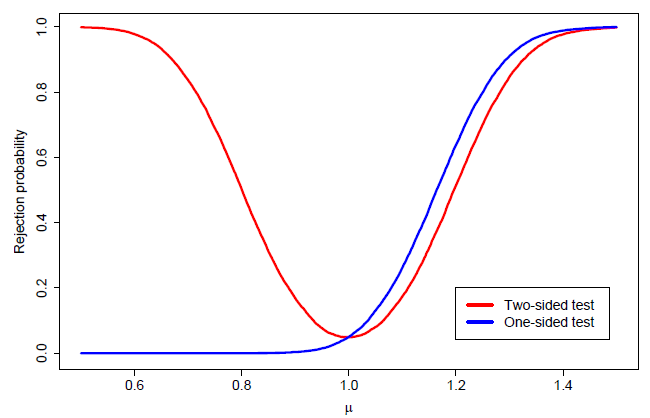
\includegraphics[width = 0.15\textwidth]{content/power_curves.png}\\
\textbf{Def (p-value)}: For any realization $T^*$, $p^* = inf\{p\in[0,1]: T^*>c_p\}$. Intuition: smallest $\alpha$ for which we would still reject. \\\footnotesize{Under $H_0$, $p\sim Unif[0,1]$ (require $P(p^*<\alpha)=\alpha$, i.e. want $Pr_\theta(reject H_0) < \alpha$), but holds $\forall\alpha$.}\\
\textbf{p-value with simple $H_0$}: If $F_0$ is strictly increasing, $p* = 1 - F_0(T*)$ (again: $p~_{H_0}Unif[0,1]$).

\footnotesize{With parametric distributions with multiple parameters (e.g. $N(\mu, \sigma^2)$) usually fix one parameter (e.g. $\sigma^2$) resulting in simple test but technically \textit{composite} $H_0$.}

\subsection{Hypothesis Testing and CIs}
\textbf{Test-inversion}: Assume test $H_0: \theta = \theta_0$ and have test s.t. $P_{\theta_0}(reject H_0) = \alpha$ (size $\alpha$). Assume can perform for any $\theta_0 in \Theta$. Then we have $CS = \{\theta_0\in\Theta: not reject H_0: \theta=\theta_0\}$ with $P_\theta(\theta\in CS) = 1-\alpha$.\\
We can also do the reverse: From any CS with coverage rate $1-\alpha$ can construct size $\alpha$ test as $reject\Leftrightarrow \theta_0\notin CS$.\\
\textbf{Ex. one-sided CI}: Testing $H_0: \mu = \mu_0$ against $H_1:\mu>\mu_0$ (or $H_0: \mu \leq \mu_0$) for normal case we have $CS = \{\mu_0 \in [\bar{X}_n - \frac{t_{1-\alpha, n-1}}{\sqrt{n}}S_n, \infty)\}$.

\subsection{Asymptotic Approximations}: 
\textbf{Asymptotic argument}: No parametric model $f_(x;\theta)$, but, e.g., moments: $H_0: E(X) = \mu$. $T\xrightarrow{d}|N(0,1)|$ and we can use $\Phi^-1(x)$ to control $\alpha$ asymptotically. In particular, $P(T>z_{1-\alpha/2})\rightarrow \alpha$ under $H_0$.\\ 
\textbf{Hypotheses}: Set of distributions $\mathbb{P}$ with $\mathbb{P}_0\subset\mathbb{P}$ set of distributions consitent with $H_0$.\\
\textbf{Def 7.7 (Asymptotic power function)}: $\beta^\alpha(P) = lim_{n\to\infty}beta_n(P)$.\\
\textbf{Def 7.8/7.9}: test with $\beta^a(P)$ is \emph{asymptotic level} $\alpha$ if $sup_{P\in P_0}\beta^a(P)\leq\alpha$ (\emph{size}: equality).\\
\textbf{Def 7.10}: Test \emph{consistent} against alternative $P\in P_1$ if $\beta^a(P) = 1$.
\section*{Distributions}
% Features: Moments, MLE, convolutions, relation to other distributions
% Normal
\textbf{Normal}: $E(X)= \mu$, $Var(X) = \sigma^2$. Sum of two independent Normals is Normal. \\
\textbf{MVN}: $\sim N(\mu, \Sigma)$. Any linear combinations are Normal. $(X,Y) \sim N(\mu, \Sigma)$, then $X\independent Y \Leftrightarrow Cov(X,Y) = 0$. \\
% Bernoulli
% \textbf{Bernoulli}: $X\sim Bern(p)$, $E(X) = E(X^k) = p$ and $Var(X) = p(1-p)$. $\hat{p}_{MLE} = \bar{X}_n$.\\
% Binomial
% Uniform
\textbf{Uniform}: $X\sim Unif(a,b)$, $F_X(x) = \frac{x-a}{b-a}$, $f_X(x) = \frac{1}{b-a}$, $E(X) = \frac{1}{2(b-a)}$, $Var(X) = \frac{1}{12}(b-a)^2$. $\hat{b}_{MLE} = max\{X_1, \ldots, X_n\}$ (min for a); $\hat{b}_{MM} = 2\bar{X}_n$.\\
\textit{Uniform Order Statistics}: $U_{(k)} \sim Beta(k, n+1-k)$ with $E(U_{(k)}) = \frac{k}{n+1}$.
% Exponential
\textbf{Exponential}: $X\sim Expo(\theta)$ then $E(X^k) = k!\theta^k$, so $E(X) = \theta$ and $Var(X) = \theta^2$. $\hat{\theta}_{MLE} = \bar{X}_n$.\\
% Pareto
\textbf{Pareto}: $X\sim Pareto(\alpha)$ then $E(X^k)$ only exists if $\alpha>k$. Given that, $E(X) = \frac{\alpha}{\alpha-1}$ and $Var(X) = \frac{\alpha}{(1-\alpha)^2(\alpha-2)}$. $Y = log(X) ~ Expo(\alpha)$. 20-80 rule: $\alpha = \frac{\ln 5}{\ln 4}\approx 1.16$.\\
% Poisson
% \textbf{Poisson}: $K\sim Poisson(\lambda)$, $f_K(k) = \frac{\lambda^k\exp^{-\lambda}}{k!}$, $\lambda \in (0, \infty)$, $k\in\mathbb{N}_0$. $\hat{\lambda}_{MLE} = \bar{X}_n$.\\
\textbf{t}: If $Y\sim N(0,1)$ and $Z\sim \chi^2_{n-1}$ and $X\independent Z$ then $\frac{N}{Z}~t_{n-1}$.\\
% Chi-square
% t-Distribution, Cauchy
\textbf{Cauchy}: $X, Y \sim N(0, 1)$ with $X\independent Y$, then $\frac{X}{Y}~Cauchy(0,1)$. Expectation and variance undefined. $X\sim Cauchy(0,1)$ then $X\sim t_1$.
% \input{content/aussagen}
% \input{content/mengen}
% \input{content/relationen}
% \input{content/abbildungen}
%\input{content/beweise} 
%\input{content/graphen}
%\input{content/graphalgo}
%\input{content/bool}
%\input{content/formeln}
\end{multicols*}
\end{document}